\documentclass{standalone}
\usepackage{tikz}
\usetikzlibrary{patterns, positioning}


\begin{document}
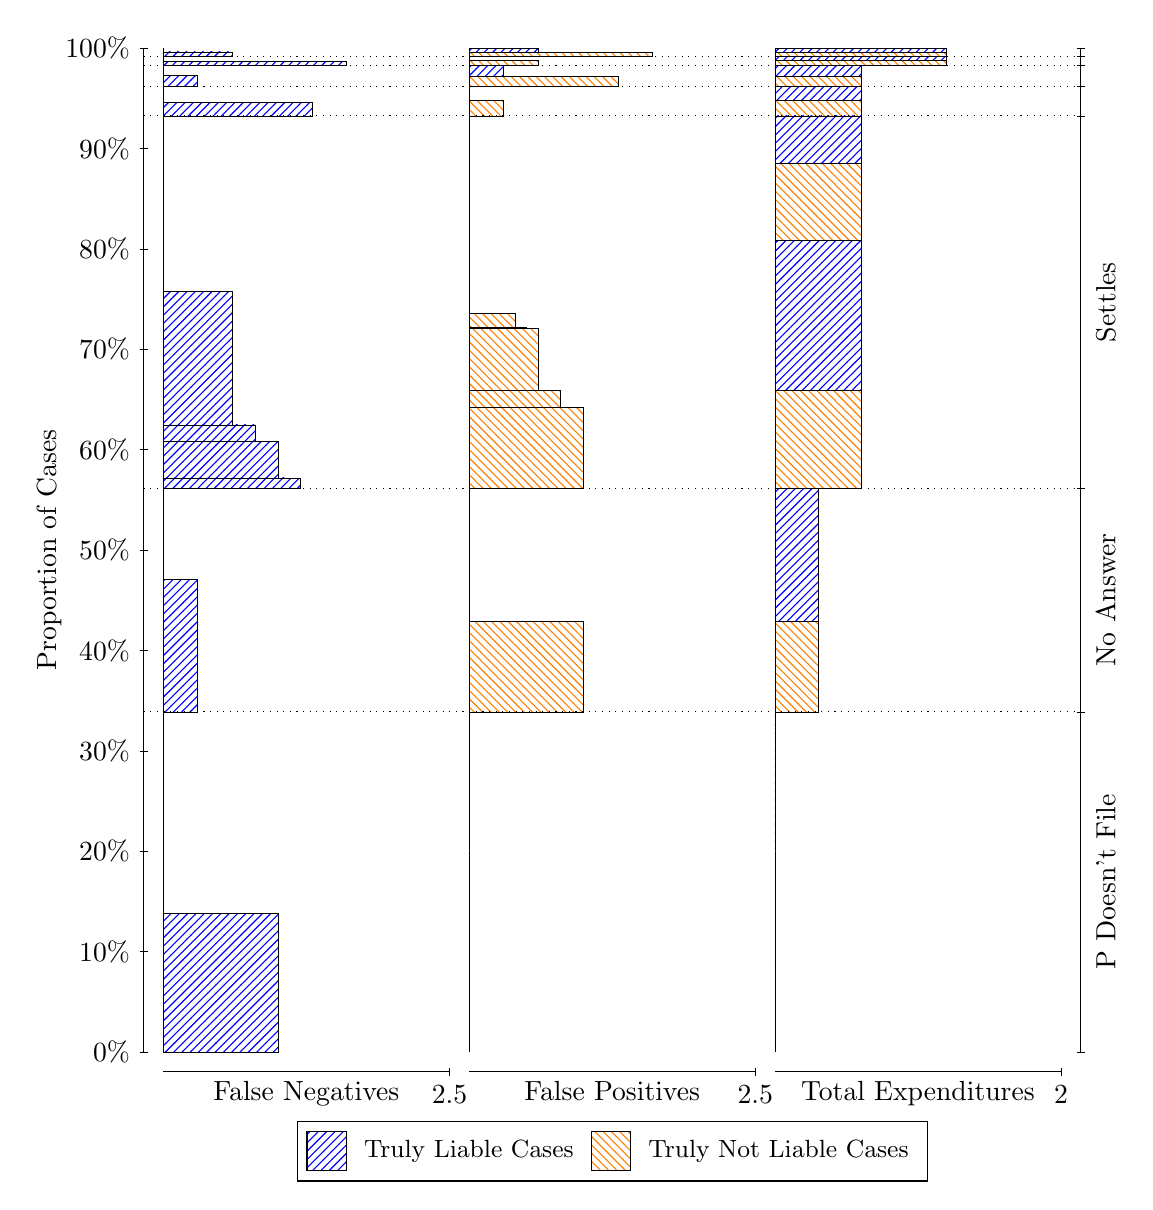
\begin{tikzpicture}
\draw[black, very thin] (1.5,1.75) -- (1.5,14.5);
\node[rotate=90, text=black, anchor=center] at (0.3, 8.125) {Proportion of Cases};
\draw[black, very thin] (1.45,1.75) -- (1.55,1.75);
\node[text=black, anchor=east] at (1.45, 1.75) {0\%};
\draw[black, very thin] (1.45,3.025) -- (1.55,3.025);
\node[text=black, anchor=east] at (1.45, 3.025) {10\%};
\draw[black, very thin] (1.45,4.3) -- (1.55,4.3);
\node[text=black, anchor=east] at (1.45, 4.3) {20\%};
\draw[black, very thin] (1.45,5.575) -- (1.55,5.575);
\node[text=black, anchor=east] at (1.45, 5.575) {30\%};
\draw[black, very thin] (1.45,6.85) -- (1.55,6.85);
\node[text=black, anchor=east] at (1.45, 6.85) {40\%};
\draw[black, very thin] (1.45,8.125) -- (1.55,8.125);
\node[text=black, anchor=east] at (1.45, 8.125) {50\%};
\draw[black, very thin] (1.45,9.4) -- (1.55,9.4);
\node[text=black, anchor=east] at (1.45, 9.4) {60\%};
\draw[black, very thin] (1.45,10.675) -- (1.55,10.675);
\node[text=black, anchor=east] at (1.45, 10.675) {70\%};
\draw[black, very thin] (1.45,11.95) -- (1.55,11.95);
\node[text=black, anchor=east] at (1.45, 11.95) {80\%};
\draw[black, very thin] (1.45,13.225) -- (1.55,13.225);
\node[text=black, anchor=east] at (1.45, 13.225) {90\%};
\draw[black, very thin] (1.45,14.5) -- (1.55,14.5);
\node[text=black, anchor=east] at (1.45, 14.5) {100\%};

\draw[black, very thin] (13.4,1.75) -- (13.4,14.5);
\draw[black, very thin] (13.35,1.75) -- (13.45,1.75);
\node[anchor=west] at (13.35, 1.75) {};
\draw[black, very thin] (13.35,6.0687) -- (13.45,6.0687);
\node[anchor=west] at (13.35, 6.0687) {};
\draw[black, very thin] (13.35,8.9079) -- (13.45,8.9079);
\node[anchor=west] at (13.35, 8.9079) {};
\draw[black, very thin] (13.35,13.638) -- (13.45,13.638);
\node[anchor=west] at (13.35, 13.638) {};
\draw[black, very thin] (13.35,14.013) -- (13.45,14.013);
\node[anchor=west] at (13.35, 14.013) {};
\draw[black, very thin] (13.35,14.281) -- (13.45,14.281);
\node[anchor=west] at (13.35, 14.281) {};
\draw[black, very thin] (13.35,14.391) -- (13.45,14.391);
\node[anchor=west] at (13.35, 14.391) {};
\draw[black, very thin] (13.35,14.5) -- (13.45,14.5);
\node[anchor=west] at (13.35, 14.5) {};

\draw[black, very thin, pattern color=blue, pattern=north east lines] (1.75,1.75) rectangle (3.2033,3.5095);
\draw[black, very thin, pattern color=orange, pattern=north west lines] (1.75,3.5095) rectangle (1.75,6.0687);
\draw[black, very thin, pattern color=blue, pattern=north east lines] (1.75,6.0687) rectangle (2.186,7.7558);
\draw[black, very thin, pattern color=orange, pattern=north west lines] (1.75,7.7558) rectangle (1.75,8.9079);
\draw[black, very thin, pattern color=blue, pattern=north east lines] (1.75,8.9079) rectangle (3.494,9.0344);
\draw[black, very thin, pattern color=blue, pattern=north east lines] (1.75,9.0344) rectangle (3.3487,9.0414);
\draw[black, very thin, pattern color=blue, pattern=north east lines] (1.75,9.0414) rectangle (3.2033,9.5081);
\draw[black, very thin, pattern color=blue, pattern=north east lines] (1.75,9.5081) rectangle (2.9127,9.715);
\draw[black, very thin, pattern color=blue, pattern=north east lines] (1.75,9.715) rectangle (2.622,11.414);
\draw[black, very thin, pattern color=orange, pattern=north west lines] (1.75,11.414) rectangle (1.75,13.638);
\draw[black, very thin, pattern color=blue, pattern=north east lines] (1.75,13.638) rectangle (3.6393,13.814);
\draw[black, very thin, pattern color=orange, pattern=north west lines] (1.75,13.814) rectangle (1.75,14.013);
\draw[black, very thin, pattern color=blue, pattern=north east lines] (1.75,14.013) rectangle (2.186,14.151);
\draw[black, very thin, pattern color=orange, pattern=north west lines] (1.75,14.151) rectangle (1.75,14.281);
\draw[black, very thin, pattern color=blue, pattern=north east lines] (1.75,14.281) rectangle (4.0753,14.33);
\draw[black, very thin, pattern color=orange, pattern=north west lines] (1.75,14.33) rectangle (1.75,14.391);
\draw[black, very thin, pattern color=blue, pattern=north east lines] (1.75,14.391) rectangle (2.622,14.452);
\draw[black, very thin, pattern color=orange, pattern=north west lines] (1.75,14.452) rectangle (1.75,14.5);
\draw[black, very thin, pattern color=orange, pattern=north west lines] (5.6333,1.75) rectangle (5.6333,4.3092);
\draw[black, very thin, pattern color=blue, pattern=north east lines] (5.6333,4.3092) rectangle (5.6333,6.0687);
\draw[black, very thin, pattern color=orange, pattern=north west lines] (5.6333,6.0687) rectangle (7.0867,7.2208);
\draw[black, very thin, pattern color=blue, pattern=north east lines] (5.6333,7.2208) rectangle (5.6333,8.9079);
\draw[black, very thin, pattern color=orange, pattern=north west lines] (5.6333,8.9079) rectangle (7.0867,9.9353);
\draw[black, very thin, pattern color=orange, pattern=north west lines] (5.6333,9.9353) rectangle (6.796,10.151);
\draw[black, very thin, pattern color=orange, pattern=north west lines] (5.6333,10.151) rectangle (6.5053,10.941);
\draw[black, very thin, pattern color=orange, pattern=north west lines] (5.6333,10.941) rectangle (6.36,10.95);
\draw[black, very thin, pattern color=orange, pattern=north west lines] (5.6333,10.95) rectangle (6.2147,11.132);
\draw[black, very thin, pattern color=blue, pattern=north east lines] (5.6333,11.132) rectangle (5.6333,13.638);
\draw[black, very thin, pattern color=orange, pattern=north west lines] (5.6333,13.638) rectangle (6.0693,13.837);
\draw[black, very thin, pattern color=blue, pattern=north east lines] (5.6333,13.837) rectangle (5.6333,14.013);
\draw[black, very thin, pattern color=orange, pattern=north west lines] (5.6333,14.013) rectangle (7.5227,14.144);
\draw[black, very thin, pattern color=blue, pattern=north east lines] (5.6333,14.144) rectangle (6.0693,14.281);
\draw[black, very thin, pattern color=orange, pattern=north west lines] (5.6333,14.281) rectangle (6.5053,14.343);
\draw[black, very thin, pattern color=blue, pattern=north east lines] (5.6333,14.343) rectangle (5.6333,14.391);
\draw[black, very thin, pattern color=orange, pattern=north west lines] (5.6333,14.391) rectangle (7.9587,14.44);
\draw[black, very thin, pattern color=blue, pattern=north east lines] (5.6333,14.44) rectangle (6.5053,14.5);
\draw[black, very thin, pattern color=orange, pattern=north west lines] (9.5167,1.75) rectangle (9.5167,4.3092);
\draw[black, very thin, pattern color=blue, pattern=north east lines] (9.5167,4.3092) rectangle (9.5167,6.0687);
\draw[black, very thin, pattern color=orange, pattern=north west lines] (9.5167,6.0687) rectangle (10.062,7.2208);
\draw[black, very thin, pattern color=blue, pattern=north east lines] (9.5167,7.2208) rectangle (10.062,8.9079);
\draw[black, very thin, pattern color=orange, pattern=north west lines] (9.5167,8.9079) rectangle (10.607,10.151);
\draw[black, very thin, pattern color=blue, pattern=north east lines] (9.5167,10.151) rectangle (10.607,12.057);
\draw[black, very thin, pattern color=orange, pattern=north west lines] (9.5167,12.057) rectangle (10.607,13.038);
\draw[black, very thin, pattern color=blue, pattern=north east lines] (9.5167,13.038) rectangle (10.607,13.638);
\draw[black, very thin, pattern color=orange, pattern=north west lines] (9.5167,13.638) rectangle (10.607,13.837);
\draw[black, very thin, pattern color=blue, pattern=north east lines] (9.5167,13.837) rectangle (10.607,14.013);
\draw[black, very thin, pattern color=orange, pattern=north west lines] (9.5167,14.013) rectangle (10.607,14.144);
\draw[black, very thin, pattern color=blue, pattern=north east lines] (9.5167,14.144) rectangle (10.607,14.281);
\draw[black, very thin, pattern color=orange, pattern=north west lines] (9.5167,14.281) rectangle (11.697,14.343);
\draw[black, very thin, pattern color=blue, pattern=north east lines] (9.5167,14.343) rectangle (11.697,14.391);
\draw[black, very thin, pattern color=orange, pattern=north west lines] (9.5167,14.391) rectangle (11.697,14.44);
\draw[black, very thin, pattern color=blue, pattern=north east lines] (9.5167,14.44) rectangle (11.697,14.5);
\draw[black, dotted] (1.5,6.0687) -- (13.4,6.0687);
\draw[black, dotted] (1.5,8.9079) -- (13.4,8.9079);
\draw[black, dotted] (1.5,13.638) -- (13.4,13.638);
\draw[black, dotted] (1.5,14.013) -- (13.4,14.013);
\draw[black, dotted] (1.5,14.281) -- (13.4,14.281);
\draw[black, dotted] (1.5,14.391) -- (13.4,14.391);
\draw[black, very thin] (1.75,1.5) -- (5.3833,1.5);
\node[text=black, anchor=north] at (3.5667, 1.5) {False Negatives};
\draw[black, very thin] (5.3833,1.45) -- (5.3833,1.55);
\node[text=black, anchor=north] at (5.3833, 1.45) {2.5};

\draw[black, very thin] (5.6333,1.5) -- (9.2667,1.5);
\node[text=black, anchor=north] at (7.45, 1.5) {False Positives};
\draw[black, very thin] (9.2667,1.45) -- (9.2667,1.55);
\node[text=black, anchor=north] at (9.2667, 1.45) {2.5};

\draw[black, very thin] (9.5167,1.5) -- (13.15,1.5);
\node[text=black, anchor=north] at (11.333, 1.5) {Total Expenditures};
\draw[black, very thin] (13.15,1.45) -- (13.15,1.55);
\node[text=black, anchor=north] at (13.15, 1.45) {2};

\node[text=black, centered, rotate=90] at (13.72, 3.9093) {P Doesn't File};
\node[text=black, centered, rotate=90] at (13.72, 7.4883) {No Answer};
\node[text=black, centered, rotate=90] at (13.72, 11.273) {Settles};





\draw (7.449999999999999,1.5) node[draw=none] (baseCoordinate) {};
\begin{scope}[align=center]
        \matrix[scale=0.5, draw=black, below=0.5cm of baseCoordinate, nodes={draw}, column sep=0.1cm]{
            \node[rectangle, draw, minimum width=0.5cm, minimum height=0.5cm, pattern color=blue, pattern=north east lines] {}; &
            \node[draw=none, font=\small, text=black] (B) {Truly Liable Cases}; &
            \node[rectangle, draw, minimum width=0.5cm, minimum height=0.5cm, pattern color=orange, pattern=north west lines] {}; &
            \node[draw=none, font=\small, text=black] (B) {Truly Not Liable Cases}; \\
            };
\end{scope}

\end{tikzpicture}
\end{document}